\documentclass[11pt,a4paper]{article}
\usepackage[T1]{fontenc}
\usepackage[utf8]{inputenc}
\usepackage[french]{babel}
\frenchsetup{SmallCapsFigTabCaptions=false}
\usepackage[autostyle]{csquotes}
\usepackage[margin=2.5cm]{geometry}
\usepackage{lmodern,microtype,booktabs,tabularx,graphicx}
\usepackage[font=small,labelfont=bf]{caption}
\usepackage[backend=biber,style=authoryear,maxcitenames=2,mincitenames=1,
  maxbibnames=6,minbibnames=3,giveninits=true,uniquename=false,uniquelist=false,
  dashed=false,doi=true,url=true,isbn=false,eprint=false]{biblatex}
\addbibresource{references.bib}
\usepackage[hidelinks]{hyperref}

\newcolumntype{L}{>{\raggedright\arraybackslash}X}

\title{Visual Reasoning Maps\\[0.3em]\large Reconstruire, montrer et vérifier le raisonnement d’un texte\\État de l’art et positionnement}
\author{Document de travail — projet ENAC}
\date{23 septembre 2026}

\begin{document}
\maketitle

\begin{abstract}
Les modèles de langage résument volontiers un article, mais un résumé ne montre ni comment les affirmations s’enchaînent ni sur quelles phrases elles reposent, et il tend à généraliser au-delà de ce que dit le texte. Visual Reasoning Maps est un prototype qui reconstruit le raisonnement d’un texte sous forme de carte : des étapes typées (question, prémisse, affirmation, preuve, objection, conclusion), reliées par des relations de soutien, de cause, de précision ou de contradiction, chacune rattachée aux phrases qui la fondent. Ce document examine 33 sources, lues pour la plupart en texte intégral, qui relèvent de la théorie de l’argumentation et de la fouille d’arguments, de la visualisation de textes à l’aide de modèles de langage, du dessin de graphes, des interfaces de lecture scientifique et du contrôle des sorties de modèles. Il en tire six exigences de conception et montre comment le prototype y répond. Dans le corpus examiné, aucun système ne réunit des relations inférentielles typées, un aperçu hiérarchique, un ancrage vérifié phrase par phrase dans la mise en page d’origine et un statut de vérification visible pour chaque élément. Le document se termine par un protocole d’évaluation, qui reste à conduire.
\end{abstract}

\tableofcontents

\section{Introduction}

\subsection{Du résumé à la reconstruction}

Lire un article, c’est repérer ce qu’il affirme, ce qui justifie chaque affirmation et les objections auxquelles il répond. Les assistants fondés sur des modèles de langage (LLM) proposent surtout des résumés. Un résumé condense le contenu, mais il ne rend pas inspectables les dépendances entre propositions. Il n’est pas non plus toujours fidèle : sur 4\,900 résumés produits par dix modèles, \textcite{ref30} observent des généralisations plus larges que celles des textes d’origine, dans 26 à 73~\% des cas pour trois des modèles étudiés, et près de cinq fois plus souvent que dans des résumés écrits par des humains. Un lecteur qui veut juger un raisonnement a besoin d’en voir la structure et de pouvoir remonter, pour chaque pas, à la phrase qui le fonde.

Le sujet du projet demande un outil de ce type : extraire d’un texte les concepts, les arguments, les exemples, les positions adverses et les conclusions ; repérer des motifs de raisonnement (divergence, convergence, contradiction, raffinement, causalité) ; les montrer sous forme de carte ou de \emph{storyline} qui suive l’évolution des idées dans le texte ; retrouver d’un clic le passage d’origine de chaque élément ; tester l’ensemble sur des textes philosophiques, scientifiques et des essais. Visual Reasoning Maps est le prototype réalisé pour y répondre. Il présente un aperçu de cinq à douze étapes, développables en sous-étapes, et affiche pour chaque étape les phrases citées dans la mise en page d’origine du document (figure~\ref{fig:prototype}).

\begin{figure}[t]
\centering
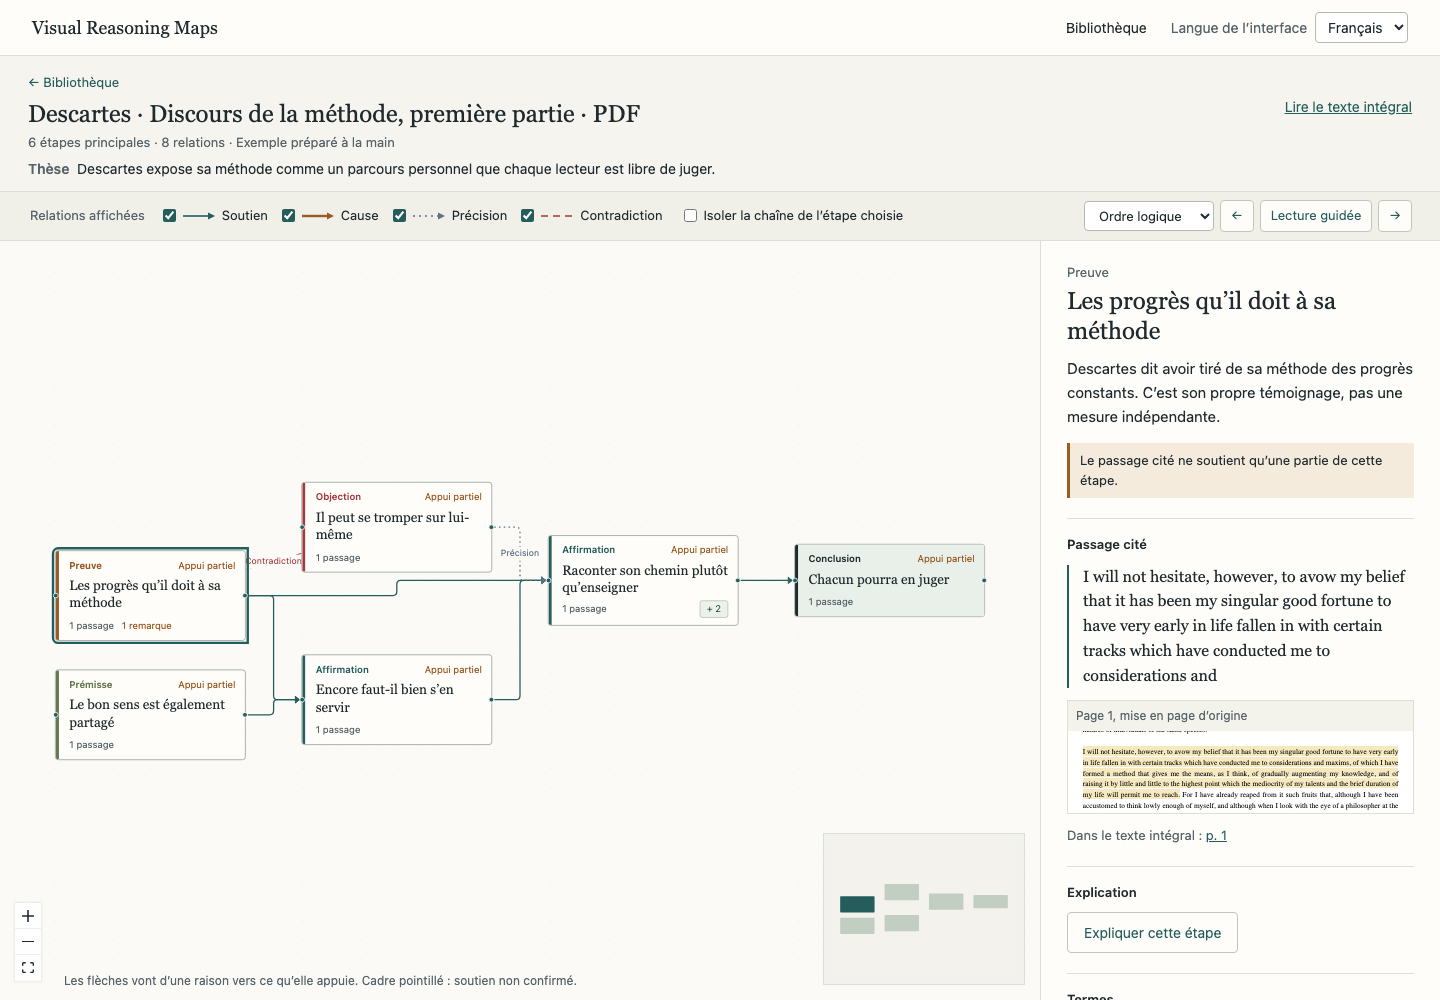
\includegraphics[width=\textwidth]{figures/carte-descartes.png}
\caption{Le prototype sur l’exemple fourni avec le dépôt, la première partie du \emph{Discours de la méthode} dans une traduction anglaise du domaine public. À gauche, la carte des étapes principales ; à droite, l’étape sélectionnée, son statut et le passage cité dans sa mise en page d’origine. Cet exemple a été préparé à la main.}
\label{fig:prototype}
\end{figure}

\subsection{Questions}

Quatre questions organisent la revue :
\begin{enumerate}
  \item Quelles unités et quelles relations extraire, et avec quelle fiabilité un modèle peut-il le faire ?
  \item Comment les disposer pour donner une vue d’ensemble sans couper le lecteur du texte ?
  \item Comment rattacher chaque élément au texte, et comment contrôler ce rattachement ?
  \item Comment évaluer un tel système, sachant que le modèle qui produit la carte ne peut pas en être le seul juge ?
\end{enumerate}

\subsection{Corpus et méthode}

Le point de départ est une liste de 23 références fixée au lancement du projet, accompagnée d’une lecture facultative, la revue de \textcite{ref12b} sur le regroupement d’arêtes, que nous avons retenue. Nous y avons ajouté huit sources pour combler des manques apparus pendant la rédaction : la théorie de l’argumentation et du discours \parencite{ref24,ref25,ref26}, un principe classique de conception d’interfaces de visualisation \parencite{ref27}, la vérification d’affirmations scientifiques \parencite{ref28}, la fiabilité des LLM employés comme juges \parencite{ref29}, la fidélité des résumés scientifiques produits par des LLM \parencite{ref30} et la documentation de l’algorithme de disposition utilisé par le prototype \parencite{ref31}. La revue n’est donc pas systématique.

Les textes ont été lus en intégralité quand ils étaient librement accessibles. Quatre ne l’ont été qu’à travers leur résumé et leurs métadonnées \parencite{ref09,ref10,ref12,ref12b} : nous ne leur prêtons rien de plus. Les références renvoient aux versions publiées ; lorsque la version lue est une prépublication, les pages citées sont celles de cette version. Chaque source a une fiche de lecture (dossier \texttt{paper/fiches} du dépôt) qui indique la version consultée, les pages utilisées et ce qui reste à vérifier. Les sources ont été consultées les 22 et 23 septembre 2026.

\subsection{Plan}

La section~\ref{sec:notions} précise ce que la carte représente. Les sections~\ref{sec:extraction} à~\ref{sec:critique} traitent successivement de l’extraction de la structure, de sa représentation, de son ancrage dans le texte et de la critique automatique. La section~\ref{sec:synthese} compare les systèmes étudiés, en tire six exigences et situe le prototype ; la section~\ref{sec:evaluation} décrit le protocole d’évaluation prévu.

\section{Ce que la carte représente}
\label{sec:notions}

\subsection{Le rôle des énoncés}

Le modèle de \textcite{ref24}, conçu à l’origine pour l’argumentation juridique, distingue six composantes d’un argument : l’affirmation, la donnée, le garant, le fondement, le modalisateur et la réfutation \parencite[41]{ref08}. Appliqué à des articles scientifiques, il s’est révélé mal adapté. Lors d’une annotation préliminaire, \textcite[41]{ref08} n’ont trouvé ni garant, ni fondement, ni modalisateur, ni réfutation ; en revanche, des affirmations servaient souvent d’appui à d’autres affirmations. Leur schéma final ne garde que trois rôles, l’affirmation propre aux auteurs, l’affirmation qui relève du contexte et la donnée, et trois relations : le soutien, la contradiction et l’identité sémantique entre deux mentions d’une même affirmation. Pour des essais argumentatifs, \textcite{ref07} retiennent la thèse, l’affirmation et la prémisse, reliées par le soutien ou l’attaque.

Le prototype adopte six rôles : question, prémisse, affirmation, preuve, objection et conclusion. Ils suivent la demande du sujet (concepts, arguments, exemples, positions adverses, conclusions) plus qu’une théorie particulière. La question marque le point de départ d’un raisonnement, la preuve regroupe données et exemples, l’objection recueille les positions que l’auteur discute. Les concepts ne deviennent pas des étapes : ils figurent dans des fiches de termes, rattachées aux étapes où ils interviennent.

\subsection{Les relations}

En fouille d’arguments, les relations se ramènent le plus souvent au soutien et à l’attaque \parencite{ref05,ref07}. Le sujet en demande davantage, car la causalité et le raffinement ne sont pas des relations d’inférence. Ils relèvent de l’organisation du discours telle que la décrit la théorie de la structure rhétorique \parencite{ref25}. Celle-ci définit par exemple les relations \emph{Evidence} (le satellite accroît la croyance du lecteur dans le noyau), \emph{Cause}, \emph{Elaboration} (le satellite apporte un détail sur un élément du noyau), \emph{Contrast} et \emph{Antithesis}. Les quatre relations du prototype, soutien, cause, précision et contradiction, correspondent à ces familles. La divergence et la convergence ne sont pas des relations mais des configurations : une affirmation d’où partent plusieurs branches, plusieurs preuves qui mènent à la même conclusion. Elles se lisent sur la forme du graphe.

Reste la forme d’ensemble. \textcite[620]{ref07} modélisent un essai comme un arbre connexe, alors que \textcite[43]{ref08} trouvent dans les articles scientifiques une forêt de graphes orientés acycliques. Le prototype retient le graphe orienté acyclique pour le soutien, la cause et la précision, et traite la contradiction à part : elle relie deux étapes sans que l’une précède l’autre.

\subsection{Carte d’arguments ou carte de concepts}

\textcite{ref26} distingue trois familles de cartes souvent confondues. La carte mentale relève de l’association, la carte conceptuelle des relations entre idées, la carte d’arguments de la structure inférentielle, c’est-à-dire de ce qui fonde une affirmation. Les graphes que des LLM extraient pour la recherche d’information (section~\ref{sec:graphes}) appartiennent à la deuxième famille. La carte du prototype appartient surtout à la troisième, mais pas entièrement : selon Davies, la carte d’arguments ne s’occupe pas des relations causales entre affirmations, alors que le sujet demande de les montrer. Nous gardons donc la cause et la précision, avec un trait distinct de celui du soutien, pour qu’un lecteur ne prenne pas une explication pour une preuve.

\section{Extraire la structure d’un raisonnement}
\label{sec:extraction}

\subsection{La fouille d’arguments}

\textcite[765]{ref05} définissent la fouille d’arguments comme l’identification et l’extraction automatiques de la structure d’inférence et de raisonnement exprimée par des arguments en langue naturelle. Ils organisent la tâche par niveaux de difficulté croissante : délimiter les composantes, qualifier les propositions, puis identifier les relations, des simples liens entre prémisse et conclusion jusqu’aux schèmes d’argumentation \parencite[786--787]{ref05}. Les outils d’analyse classiques, comme Araucaria, Rationale, OVA ou Carneades, laissent à l’analyste le soin d’identifier les propositions \parencite[775]{ref05}. Les difficultés que relèvent les auteurs tiennent surtout aux données : peu de corpus annotés, des schémas d’annotation propres à chaque domaine, des conceptions divergentes de ce qu’est une affirmation, et une part du raisonnement que le texte laisse implicite \parencite[806--807]{ref05}.

Les résultats de \textcite{ref07} donnent l’ordre de grandeur de ces difficultés. Sur un corpus de 402 essais, leur modèle joint optimise ensemble les types de composantes et les relations par programmation linéaire en nombres entiers. Il atteint un F1 macro de 0,826 pour les composantes, pour un plafond humain de 0,868, et de 0,751 pour les relations, contre 0,854. Pour les seules relations d’attaque, le F1 tombe à 0,413, contre 0,703 chez les annotateurs \parencite[646]{ref07}. L’accord entre annotateurs est lui-même plus faible pour les affirmations ($\alpha_U = 0{,}524$) que pour les prémisses ($0{,}824$) \parencite[631]{ref07}. Les relations sont donc plus difficiles à retrouver que les composantes, et l’attaque plus que le soutien.

Le texte scientifique ajoute une difficulté de portée. Dans les 40 articles annotés par \textcite[43]{ref08}, on compte en moyenne 141 composantes connexes par article, pour un diamètre moyen de 3. Les auteurs y voient soit des chaînes argumentatives très courtes, soit la difficulté, pour les annotateurs eux-mêmes, de repérer les dépendances à longue distance. Une analyse qui part des phrases pour remonter vers la structure risque ainsi de produire des fragments sans vue d’ensemble.

\subsection{Avec des modèles de langage}

La revue de \textcite{ref06} montre comment les LLM ont estompé les frontières entre sous-tâches : un même modèle, guidé par des instructions, des exemples ou une chaîne de raisonnement, détecte des affirmations, des preuves ou des positions. Elle signale aussi un risque propre à cette période : lorsque la même famille de modèles sert à annoter des données puis à évaluer des systèmes, les scores peuvent être gonflés \parencite[7]{ref06}.

Deux systèmes de visualisation mesurent la qualité de leur propre extraction. Graphologue fait annoter par GPT-4, au fil de la génération, les entités et les relations de la réponse qu’il est en train de produire. La F-mesure des relations passe de 84,77~\% à 92,39~\% après un tour de correction, et la part de relations manquantes de 20,73~\% à 9,25~\% \parencite[11]{ref02}. Story Ribbons extrait des récits littéraires des attributs et des citations ; une partie des citations produites par le modèle est inventée ou modifiée, si bien que les auteurs les comparent mot à mot au texte et remplacent celles qui n’y figurent pas \parencite[3]{ref01}. La part de citations authentiques varie de 0,85 à 0,97 selon le type de texte \parencite[4]{ref01}. Dans les deux cas, l’extraction n’est utilisable qu’avec une étape de contrôle, et ce contrôle réduit les erreurs sans les supprimer.

\subsection{Les graphes de connaissances}
\label{sec:graphes}

GraphRAG \parencite{ref13} fait extraire par un LLM des entités, des relations et des affirmations factuelles, regroupe les entités en communautés hiérarchiques et résume chacune à l’avance, afin de répondre à des questions qui portent sur tout un corpus. Sur des corpus d’environ un million de jetons, ses réponses sont plus complètes et plus diverses que celles d’une recherche de passages \parencite[1]{ref13}. LightRAG \parencite{ref14} poursuit le même but avec une recherche à deux niveaux et des mises à jour incrémentales. Les auteurs de GraphRAG précisent que l’extraction d’entités, de relations et d’affirmations est une forme de résumé abstractif : relations et affirmations peuvent ne pas être énoncées explicitement dans le texte \parencite[5]{ref13}.

Ces graphes relient des concepts pour retrouver l’information. Ils ne disent pas quelle proposition justifie laquelle, et leurs arêtes ne renvoient pas à une phrase précise. Le résumé hiérarchique des communautés rejoint en revanche notre besoin d’un aperçu à plusieurs niveaux.

\subsection{Conséquences pour le prototype}

Le prototype procède du haut vers le bas, en trois passes. La première esquisse le raisonnement principal en cinq à douze étapes à partir du texte regroupé par sections ; pour un document très long, seuls le début et la fin de chaque section sont transmis. La deuxième ajoute les sous-étapes section par section, la troisième cherche les relations entre sections. Poser la structure d’ensemble avant les détails répond au problème de portée relevé plus haut.

Chaque étape doit citer au moins une phrase par son identifiant (\texttt{p12s3} désigne la troisième phrase du douzième paragraphe), accompagné d’un court extrait. Les relations sont typées et orientées. Une contradiction exige une citation de chaque côté, puisque c’est le type de relation le moins bien extrait. Enfin, l’extraction et la critique décrite à la section~\ref{sec:critique} sont confiées au même modèle : les verdicts de la critique servent à signaler des problèmes, pas à mesurer la qualité de la carte.

\section{Représenter un raisonnement}
\label{sec:representation}

\subsection{Visualiser des arguments}

\textcite{ref09} formulent le problème central : saisir la structure hiérarchique d’un argument tout en pouvant lire le texte de ses prémisses pose des problèmes d’aperçu, de détail et de navigation. À partir d’entretiens avec des analystes d’arguments, ils ont conçu trois techniques qui combinent une visualisation d’arbre (\emph{sunburst} ou \emph{icicle}) et un affichage du contenu, intégré à la figure ou placé dans une infobulle. Les analystes jugeaient le \emph{sunburst} bon pour l’aperçu et préféraient le texte intégré ; une étude contrôlée avec 21 participants et trois tâches désigne pourtant le \emph{sunburst} avec infobulle comme le meilleur compromis. La tension entre aperçu et lecture n’a donc pas de solution unique : elle se règle selon la tâche. Ces arguments sont des arbres, ce qui autorise des représentations par remplissage de l’espace ; les nôtres sont des graphes avec des liens transversaux et des contradictions, d’où le choix d’une représentation nœuds-liens.

\subsection{Du texte à la carte avec des LLM}

Trois systèmes récents associent extraction par LLM et visualisation interactive. Story Ribbons \parencite{ref01} trace les trajectoires des personnages et des thèmes à plusieurs niveaux narratifs pour 36 œuvres. Ses trois motifs d’interaction, les explications à la demande, les dimensions définies en langage naturel et les questions posées au modèle, sont conçus pour pallier les limites des systèmes fondés sur l’IA \parencite[1, 5]{ref01}. Parmi les 16 participants de l’étude, 14 disent pourtant que les comportements inattendus du modèle n’ont pas entamé leur confiance dans les visualisations \parencite[8]{ref01}. Une erreur visible ne rend donc pas le lecteur prudent de lui-même : ce qui n’a pas été vérifié doit être signalé comme tel.

Graphologue \parencite{ref02} transforme les réponses de GPT-4 en diagrammes nœuds-liens construits en direct ; le survol d’un nœud surligne le passage correspondant de la réponse, et inversement \parencite[8]{ref02}. Son étude utilisateur porte sur sept personnes \parencite[2]{ref02}. Sensecape \parencite{ref03} organise l’exploration d’un sujet en niveaux d’abstraction, avec un zoom sémantique et une vue hiérarchique. Dans une étude intra-sujets à 12 participants, ceux-ci explorent davantage de concepts qu’avec une interface de référence associant conversation et toile simple (68,3 contre 22,8 en moyenne) \parencite[9--10]{ref03}. Les auteurs ont volontairement omis l’indication des sources, pour ne pas distraire les participants, et écrivent qu’un déploiement réel exigerait des mécanismes pour vérifier ce que produit le modèle \parencite[14]{ref03}.

La revue de \textcite{ref04} élargit ce constat. Sur 48 systèmes qui associent LLM et visualisation, 25 ont fait l’objet d’une évaluation avec des utilisateurs \parencite[17]{ref04}, et peu d’articles ont mesuré ou cherché à améliorer la fiabilité des informations produites par le modèle. Les auteurs y voient un obstacle à l’adoption de ces outils et plaident pour un cadre d’évaluation qui prenne en compte la confiance \parencite[20]{ref04}.

\subsection{Principes d’interaction}

Le principe formulé par \textcite[336]{ref27}, d’abord l’aperçu, puis le zoom et le filtre, enfin les détails à la demande, décrit presque terme à terme l’organisation du prototype. L’aperçu montre cinq à douze étapes principales, et chaque étape se déplie en sous-étapes. Des cases filtrent les types de relations, et une option estompe tout ce qui n’appartient pas à la chaîne de l’étape choisie. Le panneau de détails présente les phrases citées, l’extrait dans sa mise en page d’origine, les termes et les remarques. La taxonomie de Shneiderman comporte aussi la tâche \enquote{relier}, qui correspond ici au passage d’une étape à ce qui l’appuie.

\subsection{Disposer le graphe}

Pour placer les étapes, le prototype utilise ELK Layered, qui met en œuvre l’approche en couches de \textcite{ref10} : les nœuds sont affectés à des couches, les couches sont réordonnées pour réduire les croisements, puis les coordonnées sont calculées \parencite{ref31}. Cette approche oriente le plus d’arêtes possible dans une même direction, ce qui convient à une lecture qui va des raisons vers les conclusions. Les contradictions n’entrent pas dans cet ordre. L’ordre du texte n’est pas perdu pour autant : la lecture guidée peut suivre l’ordre des phrases, et la page du texte intégral situe chaque étape principale dans une marge.

Le sujet évoque aussi des représentations de type \emph{storyline}, qui montrent l’évolution d’entités au fil d’un récit. StoryFlow formule leur disposition comme une optimisation hybride, discrète puis continue, qui réduit les croisements, les ondulations et l’espace perdu assez vite pour permettre l’interaction en temps réel \parencite[2436]{ref11a}. iStoryline montre que ces critères géométriques ne suffisent pas à produire ce que des personnes dessineraient à la main, et intègre des interactions de l’utilisateur dans l’optimisation \parencite[769]{ref11b}. Un axe logique n’est cependant pas une chronologie : le prototype garde la disposition en couches pour la carte et réserve l’ordre du texte à la lecture guidée et à la marge du texte intégral. Une vue de type \emph{storyline}, où chaque étape serait placée selon sa position dans le texte, reste à construire.

Le regroupement d’arêtes (\emph{edge bundling}) simplifie le dessin des graphes denses en rapprochant les arêtes semblables \parencite{ref12b}. La méthode de \textcite{ref12} construit une carte de densité des arêtes par estimation à noyau, puis déplace les arêtes le long du gradient de cette densité. Avec cinq à douze étapes, chaque relation reste lisible sans regroupement, et chacune doit pouvoir être vérifiée isolément. Le regroupement deviendrait utile si l’on dépliait de nombreuses sous-étapes à la fois ou si l’on superposait les cartes de plusieurs documents.

\section{Relier la carte au texte}
\label{sec:ancrage}

\subsection{Citer n’est pas prouver}

ALCE évalue des réponses générées avec citations selon trois dimensions : la fluidité, l’exactitude et la qualité des citations, cette dernière mesurée par un modèle d’inférence textuelle qui vérifie si les passages cités impliquent ce qui est affirmé \parencite[6466]{ref17}. Sur le jeu de données ELI5, même les meilleurs modèles n’ont pas de citations qui soutiennent entièrement leur réponse dans environ la moitié des cas \parencite[6465]{ref17}. Une citation bien placée ne garantit donc pas le soutien. SciFact pose la question dans les termes les plus proches des nôtres : décider si des résumés d’articles soutiennent ou réfutent une affirmation scientifique, et désigner les phrases qui justifient cette décision \parencite[7534]{ref28}.

Le prototype sépare ainsi deux contrôles. Le premier est mécanique : l’extrait cité doit se retrouver dans la phrase désignée par son identifiant, par comparaison approximative avec un seuil réglable ; si l’identifiant ne convient pas, l’extrait est recherché dans tout le texte. Le second est un jugement : un appel distinct du modèle décide si les phrases citées soutiennent l’étape ou la relation, entièrement, en partie ou pas du tout. Chaque élément reçoit un statut, \enquote{vérifié}, \enquote{appui partiel} ou \enquote{à vérifier}, qui s’affiche sur la carte ; ce qui reste douteux après deux tours de correction apparaît dans un cadre en pointillés. Story Ribbons pratique le même contrôle littéral pour ses citations \parencite[3]{ref01}.

\subsection{Lire dans le document}

Le projet Semantic Reader \parencite{ref15} a exploré, à travers dix prototypes étudiés avec plus de 300 participants, comment augmenter un article sans le remplacer, y compris au-dessus des PDF existants \parencite[1]{ref15}. ScholarPhi affiche la définition des termes et des symboles dans des infobulles, Scim surligne les passages selon leur fonction dans le discours, Paper Plain propose des résumés en langage simple de certains passages \parencite[4--6]{ref15}. Les fiches de termes du prototype et le surlignage des passages cités dans le texte intégral relèvent de cette famille. SciDaSynth \parencite{ref16} applique le même principe à l’extraction de données : chaque valeur extraite par le LLM reste liée à sa source, pour être validée, corrigée ou affinée. Dans une étude intra-sujets avec 24 chercheurs, les participants obtiennent des données de bonne qualité en nettement moins de temps qu’avec les méthodes de référence \parencite[2, 10]{ref16}.

Voir le passage dans sa mise en page d’origine aide le lecteur à le reconnaître et à le situer dans la page, près d’une figure ou dans une colonne. C’est pourquoi le prototype affiche l’extrait rendu depuis le PDF plutôt qu’une simple chaîne de caractères. Cela aide à juger une étape ; cela ne prouve pas la relation proposée.

\subsection{Accéder au texte}

Tout ce qui précède dépend de la lecture du document. GROBID convertit les PDF scientifiques en XML/TEI (en-tête, références, corps du texte) à l’aide de champs conditionnels aléatoires ou, en option, de réseaux profonds \parencite{ref22}. Docling s’appuie sur un modèle d’analyse de mise en page, entraîné notamment sur DocLayNet, et sur le modèle TableFormer pour les tableaux ; il reconstitue l’ordre de lecture \parencite[2--3]{ref23}. Le prototype utilise PyMuPDF, qui fournit les coordonnées de chaque mot : elles sont indispensables pour surligner une phrase dans la page. GROBID peut s’y ajouter pour enrichir la structure.

Trois sources d’erreur se cumulent : l’ordre de lecture, le découpage en phrases et l’interprétation. Une carte bien dessinée ne corrige aucune d’elles. Le premier essai du prototype sur un article de 14 pages en deux colonnes l’a montré : faute de règles de mise en page, des graduations de graphiques et des fragments de formules étaient pris pour des titres de section, et les deux colonnes se mélangeaient. Le prototype reconstitue désormais l’ordre des colonnes, repère les titres d’après la taille et la graisse des caractères, écarte figures, tableaux et formules, et recolle les phrases coupées par un changement de colonne ou de page. Les tableaux sans filets, les mises en page à trois colonnes et les PDF numérisés restent hors de portée ; un texte trop peu extractible déclenche un message explicite.

\section{Critique automatique et fiabilité des juges}
\label{sec:critique}

\subsection{La relecture automatique}

\textcite{ref18} ont comparé les commentaires de GPT-4 aux rapports de relecture de 3\,096 articles de revues du groupe Nature et de 1\,709 articles soumis à ICLR. Les points soulevés se recouvrent à 30,85~\% et 39,23~\% respectivement, un niveau comparable à celui qu’on observe entre deux relecteurs humains. Dans leur étude auprès de 308 chercheurs, 57,4~\% jugent ces retours utiles ou très utiles et 82,4~\% les trouvent plus utiles que ceux d’au moins certains relecteurs humains. GPT-4 revient cependant souvent aux mêmes types de remarques, par exemple la demande d’expériences sur d’autres jeux de données \parencite[1]{ref18}. MARG \parencite{ref19} répartit la lecture d’un article entre plusieurs instances du modèle, dont des agents spécialisés par aspect. La part de commentaires jugés génériques passe de 60~\% à 29~\%, et le nombre de bons commentaires par article est multiplié par 2,2 \parencite[1]{ref19}.

La revue de \textcite{ref20} range parmi les défis ouverts la correction des hallucinations et la résistance aux entrées conçues pour obtenir des conclusions contraires à l’intégrité scientifique \parencite[25--26]{ref20}. La page technique du Stanford Agentic Reviewer \parencite{ref21} annonce une corrélation de 0,42 entre ses notes et celles d’un relecteur, contre 0,41 entre deux relecteurs, sur des soumissions à ICLR 2025 ; il s’agit d’une documentation d’ingénierie, sans évaluation indépendante.

Ces travaux portent sur des retours qui concernent un article entier. Le prototype en tire deux choix. Ses remarques sont attachées à une étape et à des phrases précises, et il ne calcule aucune note globale de qualité scientifique. Le texte du document est traité comme un matériau à analyser, jamais comme une instruction adressée au modèle.

\subsection{Le modèle comme juge}

Employer un LLM pour juger des sorties de LLM expose à des biais connus. \textcite[1]{ref29} décrivent des biais de position, de verbosité et d’auto-complaisance, le modèle favorisant ses propres réponses ; ils mesurent aussi plus de 80~\% d’accord entre GPT-4 et des préférences humaines, autant qu’entre deux humains. Cet accord porte sur des préférences entre réponses ; il ne dit rien d’un jugement de soutien entre une phrase et une étape. Le risque de circularité signalé par \textcite[7]{ref06} s’applique directement au prototype, où la critique est faite par le même modèle que l’extraction : elle peut repérer des incohérences, mais ses erreurs ne sont pas indépendantes de celles de l’extracteur.

Les règles de structure du prototype ne dépendent pas de ce jugement. Elles signalent une affirmation ou une conclusion que rien n’appuie sur la carte, une preuve qui n’appuie aucune étape, et chaque contradiction, que le lecteur doit examiner. Une conclusion dont le soutien n’est pas confirmé fait l’objet d’une remarque qui invite à vérifier qu’elle ne va pas plus loin que les éléments cités : c’est la réponse du prototype à la surgénéralisation mesurée par \textcite{ref30}. Des remarques du modèle s’y ajoutent, rattachées elles aussi à des étapes et à des phrases.

\section{Synthèse et positionnement}
\label{sec:synthese}

\subsection{Comparaison des systèmes}

Le tableau~\ref{tab:systemes} compare les systèmes étudiés selon cinq critères : ce qu’ils prennent en entrée, ce qu’ils extraient, la forme visuelle, la manière de renvoyer à la source et l’évaluation publiée. Il ne retient que ce que les sources décrivent.

\begin{table}[ht]
\centering\footnotesize
\caption{Systèmes étudiés et prototype.}
\label{tab:systemes}
\renewcommand{\arraystretch}{1.2}
\begin{tabularx}{\textwidth}{@{}>{\raggedright\arraybackslash}p{2.7cm}LLLLL@{}}
\toprule
Système & Entrée & Structure extraite & Forme visuelle & Renvoi à la source & Évaluation publiée \\
\midrule
Story Ribbons\newline\parencite{ref01} & Romans, pièces, poèmes & Personnages, lieux, thèmes, scènes & \emph{Storylines} à plusieurs niveaux & Citations contrôlées mot à mot & Pipeline sur 36 œuvres ; 16 participants \\
Graphologue\newline\parencite{ref02} & Réponses de GPT-4 & Entités et relations & Diagrammes nœuds-liens & Passage de la réponse générée & Évaluation technique ; 7 participants \\
Sensecape\newline\parencite{ref03} & Exploration avec un LLM & Niveaux d’abstraction & Toile et vue hiérarchique & Aucun, par choix & Intra-sujets, 12 participants \\
Visualisations d’arguments\newline\parencite{ref09} & Arguments déjà analysés & Hiérarchie de prémisses & \emph{Sunburst}, \emph{icicle} & Texte des prémisses & Analystes ; 21 participants \\
GraphRAG\newline\parencite{ref13} & Corpus d’environ un million de jetons & Entités, relations, affirmations, communautés & Aucune (réponses textuelles) & Résumés abstractifs, sans renvoi à la phrase & Complétude et diversité des réponses \\
Semantic Reader\newline\parencite{ref15} & Articles en PDF & Termes, citations, fonctions du discours & Aides intégrées au document & Le document lui-même & Dix prototypes, plus de 300 participants \\
SciDaSynth\newline\parencite{ref16} & Articles scientifiques & Données tabulaires & Tables et résumés visuels & Chaque donnée liée à sa source & Intra-sujets, 24 chercheurs \\
MARG\newline\parencite{ref19} & Articles & Commentaires de relecture & Texte & Commentaires sur l’article & Étude utilisateur, 9 chercheurs \\
\addlinespace
Prototype & PDF, HTML d’arXiv & Étapes typées, relations inférentielles et discursives & Carte en couches, sous-étapes dépliables & Phrase citée, extrait dans la mise en page d’origine, statut de vérification & À conduire (section~\ref{sec:evaluation}) \\
\bottomrule
\end{tabularx}
\end{table}

Dans ce corpus, les systèmes qui visualisent des extractions de LLM ne représentent pas de relations d’inférence ; les travaux sur la visualisation d’arguments partent d’arguments déjà analysés à la main ; les interfaces de lecture ancrent leurs aides dans le document sans en reconstruire le raisonnement ; la relecture automatique produit du texte sans structure. La combinaison que vise le prototype, des relations typées, un aperçu hiérarchique, un ancrage vérifié phrase par phrase dans la mise en page d’origine et un statut visible pour chaque élément, n’apparaît dans aucun d’eux. Le corpus a été présélectionné et la revue n’est pas systématique : d’autres systèmes peuvent réunir ces éléments.

\subsection{Six exigences}

Les sections précédentes conduisent à six exigences de conception.
\begin{description}
  \item[E1. Des relations typées et orientées.] Une carte de raisonnement doit dire quelle proposition appuie, cause, précise ou contredit laquelle, ce que ne fait pas un graphe d’association \parencite{ref26,ref13}.
  \item[E2. L’ensemble avant le détail.] Un aperçu de taille limitée, développable, qui pose la structure d’ensemble avant les détails locaux \parencite{ref27,ref03,ref08}.
  \item[E3. Un ancrage vérifiable à la phrase.] Chaque élément renvoie à des phrases précises, montrées dans leur contexte d’origine, et ce renvoi est contrôlé \parencite{ref17,ref28,ref15}.
  \item[E4. L’incertitude visible.] Ce qui n’a pas été confirmé ne doit pas paraître certain, puisqu’une erreur visible n’entame pas d’elle-même la confiance \parencite{ref01,ref04}.
  \item[E5. Une critique ciblée.] Des remarques attachées à des passages plutôt qu’une note globale \parencite{ref18,ref19,ref30}.
  \item[E6. Une évaluation indépendante du modèle.] Le modèle qui produit la carte ne peut pas en être le seul juge \parencite{ref06,ref29}.
\end{description}

\subsection{Réponses du prototype}

Le tableau~\ref{tab:exigences} résume comment le prototype répond à chaque exigence et ce qui lui manque ; son interface est montrée à la figure~\ref{fig:prototype}.

\begin{table}[ht]
\centering\footnotesize
\caption{Exigences et état du prototype.}
\label{tab:exigences}
\renewcommand{\arraystretch}{1.2}
\begin{tabularx}{\textwidth}{@{}>{\raggedright\arraybackslash}p{2.4cm}LL@{}}
\toprule
Exigence & Mise en œuvre & Limites actuelles \\
\midrule
E1 Relations & Six rôles, quatre relations au trait distinct ; contradictions hors de l’ordre des couches & Cause et précision ne sont pas des relations d’inférence ; leur attribution dépend du modèle \\
E2 Ensemble & Esquisse de cinq à douze étapes, puis sous-étapes par section ; filtres et chaîne isolée & Pas encore de vue selon la position dans le texte \\
E3 Ancrage & Identifiant de phrase et extrait, contrôlés par comparaison approximative ; extrait rendu depuis le PDF ; texte intégral surligné & Erreurs de lecture des PDF difficiles (tableaux sans filets, trois colonnes, numérisation) \\
E4 Incertitude & Statut par étape et par relation, cadre en pointillés, rapport des lacunes de structure & Statuts attribués par le modèle qui a produit la carte \\
E5 Critique & Règles de structure et remarques du modèle, attachées à une étape et à des phrases ; aucune note globale & Utilité non mesurée \\
E6 Évaluation & Protocole prévu (section~\ref{sec:evaluation}) & Aucune évaluation humaine à ce jour \\
\bottomrule
\end{tabularx}
\end{table}

Un premier essai en conditions réelles donne un ordre de grandeur. Sur un article de 14 pages en deux colonnes, une analyse complète a demandé environ quatre minutes et 26 appels au modèle ; 39 des 41 étapes y ont été jugées soutenues par leurs citations. Ce chiffre vient du vérificateur lui-même : il indique que la chaîne fonctionne, pas que la carte est juste.

\section{Protocole d’évaluation}
\label{sec:evaluation}

Rien de ce qui précède ne montre que la carte aide à lire. Le protocole qui suit est prévu ; aucun résultat n’est encore disponible.

\paragraph{Qualité de la reconstruction.}
Une dizaine de textes couvrant les trois genres du sujet, articles scientifiques, textes philosophiques et essais, seront annotés indépendamment par deux personnes : étapes principales, relations et phrases d’appui. L’accord entre annotateurs sera mesuré avant toute comparaison avec le modèle, car il peut être faible pour les affirmations \parencite[631]{ref07} et les dépendances à longue distance échappent aux annotateurs eux-mêmes \parencite[43]{ref08}. On mesurera ensuite, pour chaque carte produite, la correspondance des étapes avec l’annotation, la justesse du type et du sens des relations, et la part des ancrages qui soutiennent réellement leur étape. Cette dernière mesure servira aussi à calibrer les statuts : parmi les éléments marqués \enquote{vérifié}, quelle part l’est aussi pour les annotateurs ?

\paragraph{Utilité pour la lecture.}
Une étude intra-sujets comparera trois conditions : le texte seul, le texte accompagné d’un résumé produit par le même modèle, et le texte accompagné de la carte. Les tâches consisteront à retrouver la phrase qui appuie une affirmation donnée, à repérer une conclusion insuffisamment soutenue et à répondre à des questions sur la structure du raisonnement. On mesurera l’exactitude, le temps et la confiance déclarée, rapportée à l’exactitude. Une confiance élevée sur des réponses fausses serait un mauvais signe, compte tenu de ce qu’a observé Story Ribbons \parencite[8]{ref01}.

\paragraph{Menaces à la validité.}
Trois points appellent une attention particulière. La familiarité avec les textes : Story Ribbons laissait chaque participant choisir une œuvre qu’il connaissait \parencite[7]{ref01}, ce qui facilite le jugement des sorties du modèle mais ne représente pas la lecture d’un texte nouveau. L’effet de nouveauté et la brièveté des séances, que les auteurs de Sensecape signalent comme limites de leur propre étude \parencite[13]{ref03}. Enfin, la variabilité des sorties du modèle d’une exécution à l’autre, qui rend difficile toute évaluation quantitative globale \parencite[17]{ref04} : les cartes utilisées dans l’étude seront figées à l’avance, et leur variabilité mesurée séparément.

\section{Conclusion}
\label{sec:conclusion}

Les travaux examinés fournissent les pièces du problème, dispersées entre plusieurs domaines. La fouille d’arguments montre que les relations sont plus difficiles à retrouver que les composantes, et que la structure à longue distance échappe à une analyse phrase par phrase. Les systèmes qui visualisent des extractions de LLM montrent qu’une extraction n’est utilisable qu’avec des boucles de contrôle, et que les utilisateurs gardent leur confiance même lorsqu’ils voient des erreurs. Les interfaces de lecture montrent comment augmenter un document sans le remplacer. Les travaux sur les citations et sur les LLM employés comme juges rappellent qu’une citation n’est pas une preuve et qu’un modèle ne peut pas être le seul juge de ce qu’il produit.

Visual Reasoning Maps réunit ces leçons dans une même interface : une carte de taille limitée, des relations typées, un renvoi vérifié à la phrase et un statut visible pour chaque élément. Reste la question que seul le protocole d’évaluation peut trancher : la carte aide-t-elle le lecteur à juger un raisonnement, ou lui donne-t-elle seulement l’impression de l’avoir compris ?


\printbibliography[heading=bibintoc,title={Références}]
\end{document}
